\documentclass[UTF8,fontset=fandol,zihao=5]{ctexart}

\usepackage[a4paper,margin=2cm]{geometry}
\usepackage{amsmath,amssymb,mathtools,bm,esint}
\usepackage{booktabs,tabularx,array,longtable,multirow}
\usepackage{xcolor}
\usepackage[most]{tcolorbox}
\usepackage{tikz}
\usetikzlibrary{
  positioning,
  calc,
  decorations.pathreplacing,
  arrows.meta
}

\usepackage{listings}
\usepackage{enumitem}
\usepackage{indentfirst}
\usepackage{fancyhdr}
\usepackage{hyperref}


% relationbox 中知识关系图的统一样式
\tikzset{
  relnode/.style={
    font=\small,
    align=center
  },
  relline/.style={
    thick
  },
  relarrow/.style={
    -{Stealth},
    thick
  }
}

\DeclareTextFontCommand{\textbf}{\heiti\color{main}}

\definecolor{main}{HTML}{A4374E}
\definecolor{mainlight}{HTML}{FFFFFF}
\definecolor{method}{HTML}{A46E79}
\definecolor{methodlight}{HTML}{FFF0F0}

\hypersetup{colorlinks=true,linkcolor=main,urlcolor=main}
\setlength{\parindent}{2em}
\linespread{1.5}
\setlength{\abovedisplayskip}{5pt}
\setlength{\belowdisplayskip}{5pt}
\setlength{\abovedisplayshortskip}{3pt}
\setlength{\belowdisplayshortskip}{3pt}
\setlist[itemize]{leftmargin=2em,itemsep=0.1em,topsep=0.2em}
\setlist[enumerate]{leftmargin=2.3em,itemsep=0.1em,topsep=0.2em}

\ctexset{
  section={format=\centering\heiti\zihao{3}\color{main},
           name={第,章},number=\chinese{section},aftername=\quad,
           beforeskip=0.9em,afterskip=0.5em},
  subsection={format=\heiti\zihao{5}\color{main},
              name={,、},number=\chinese{subsection},aftername=,
              beforeskip=0.6em,afterskip=0.22em},
  subsubsection={format=\heiti\zihao{5}\color{main},
                 number={（\chinese{subsubsection}）},aftername=,
                 beforeskip=0.55em,afterskip=0.15em}
}

\newtcolorbox{relationbox}{
  enhanced,breakable,colback=mainlight,colframe=main,
  boxrule=0.65pt,arc=1.4mm,left=2mm,right=2mm,top=1.2mm,bottom=1.2mm
}
\newtcolorbox{methodbox}[1][]{
  enhanced,breakable,colback=methodlight,colframe=method,
  boxrule=0.65pt,arc=1.4mm,left=2mm,right=2mm,top=1.2mm,bottom=1.2mm,
  title=#1,fonttitle=\kaishu,fontupper=\kaishu,
  before upper={\setlength{\parindent}{2em}}
}

\newtcolorbox{method}[1][]{
  enhanced,breakable,colback=methodlight,colframe=method,
  boxrule=0.65pt,arc=1.4mm,left=2mm,right=2mm,top=1.2mm,bottom=1.2mm,
  title={【题型】#1},fonttitle=\kaishu\bfseries
}

\newcommand{\R}{\mathbb{R}}
\newcommand{\N}{\mathbb{N}}
\newcommand{\dd}{\mathop{}\!\mathrm{d}}
\newcommand{\norm}[1]{\left\lVert#1\right\rVert}
\newcommand{\inner}[2]{\left\langle#1,#2\right\rangle}

\begin{document}

\begin{center}
  {\heiti\zihao{1}\color{main} 实分析笔记}\\[0.6em]
  {\kaishu 榆枋下}
\end{center}

\begin{relationbox}
\centering

\begin{tikzpicture}

% =========================================================
% 第一层：Euclid 空间、实数理论
% 垂直中心 y = 0
% =========================================================

\node[relnode] (euclid) at (0, 0.70)
  {Euclid 空间};

\node[relnode] (real) at (0,-0.70)
  {实数理论};


% 第一层汇聚
% 两条水平线 + 一条竖线，中心严格位于 y=0

\coordinate (merge1top) at (1.45, 0.70);
\coordinate (merge1mid) at (1.45, 0);
\coordinate (merge1bot) at (1.45,-0.70);

\draw[relline]
  (euclid.east) -- (merge1top);

\draw[relline]
  (real.east) -- (merge1bot);

\draw[relline]
  (merge1top) -- (merge1bot);


% =========================================================
% 第二层：极限与连续
% 垂直中心 y = 0
% =========================================================

\node[relnode] (limit) at (3.35,0)
  {极限\\与连续};

\draw[relarrow]
  (merge1mid) -- (limit.west);


% =========================================================
% 第三层：微分学、积分学
% 关于 y=0 对称
% =========================================================

\node[relnode] (diff) at (6.00, 0.70)
  {微分学};

\node[relnode] (integ) at (6.00,-0.70)
  {积分学};


% 第二层 → 第三层分叉

\coordinate (branch1) at (4.70,0);
\coordinate (branch1top) at (4.70, 0.70);
\coordinate (branch1bot) at (4.70,-0.70);

\draw[relline]
  (limit.east) -- (branch1);

\draw[relline]
  (branch1top) -- (branch1bot);

\draw[relarrow]
  (branch1top) -- (diff.west);

\draw[relarrow]
  (branch1bot) -- (integ.west);


% =========================================================
% 第三层汇聚
% 中心仍为 y=0
% =========================================================

\coordinate (merge3top) at (7.25, 0.70);
\coordinate (merge3mid) at (7.25,0);
\coordinate (merge3bot) at (7.25,-0.70);

\draw[relline]
  (diff.east) -- (merge3top);

\draw[relline]
  (integ.east) -- (merge3bot);

\draw[relline]
  (merge3top) -- (merge3bot);


% =========================================================
% 第四层
% 三个节点关于 y=0 对称
% =========================================================

\node[relnode] (ode) at (10.60, 1.35)
  {常微分方程};

\node[relnode] (analysis) at (10.60,0)
  {向量分析与场论};

\node[relnode] (series) at (10.60,-1.35)
  {无穷级数};


% 第三层 → 第四层分叉

\coordinate (branch2) at (8.55,0);
\coordinate (branch2top) at (8.55, 1.35);
\coordinate (branch2bot) at (8.55,-1.35);

% 主干
\draw[relline]
  (merge3mid) -- (branch2);

% 竖直分叉线
\draw[relline]
  (branch2top) -- (branch2bot);

% 三条输出
\draw[relarrow]
  (branch2top) -- (ode.west);

\draw[relarrow]
  (branch2) -- (analysis.west);

\draw[relarrow]
  (branch2bot) -- (series.west);


\end{tikzpicture}

\end{relationbox}

\section{前置知识}

均值不等式：
\[
\frac{n}{\displaystyle\sum_{k=1}^{n}\frac{1}{x_k}}
\leq \sqrt[n]{\prod_{k=1}^{n}x_k}
\leq \frac{1}{n}\sum_{k=1}^{n}x_k
\leq \sqrt{\frac{1}{n}\sum_{k=1}^{n}x_k^2},
\]
当且仅当 $x_1=x_2=\cdots=x_n$ 时取等。

二维形式：
\[
\frac{2ab}{a+b}\leq\sqrt{ab}\leq\frac{a+b}{2}
\leq\sqrt{\frac{a^2+b^2}{2}},
\]
当且仅当 $a=b$ 时取等。

Cauchy--Schwarz 不等式：
\[
|\inner{\bm{x}}{\bm{y}}|\leq\norm{\bm{x}}\,\norm{\bm{y}},
\]
当且仅当 $\bm{x}=k\bm{y}$ 时取等。

二维形式：
\[
(ac+bd)^2\leq(a^2+b^2)(c^2+d^2),
\]
当且仅当 $ad=bc$ 时取等。

\section{Euclid 空间}

本书绝大部分概念与理论建立在 Euclid 空间的基础上，故先简单介绍 Euclid 空间。理解 Euclid 空间有利于后续学习微积分时建立直观理解。

Euclid 空间建立于 $n$ 维实向量空间 $\R^n$ 中。$\R^n$ 与下列运算共同组成 Euclid 空间：

\begin{enumerate}
  \item 加法：$\bm{u}+\bm{v}\in\R^n$；
  \item 数乘：$C\bm{u}\in\R^n$；
  \item 内积：
  \[
  \inner{\bm{u}}{\bm{v}}=\sum_{i=1}^{n}u_iv_i\in\R,
  \]
  满足对称性、线性与正定性。
\end{enumerate}

加法与数乘均满足线性空间八条公理，此处不赘述。由内积定义：

\begin{enumerate}
  \item 长度（模、范数）：
  \[
  \norm{\bm{u}}=\sqrt{\inner{\bm{u}}{\bm{u}}},
  \qquad d(\bm{u},\bm{v})=\norm{\bm{u}-\bm{v}};
  \]
  \item 角度：
  \[
  \theta=\arccos\frac{\inner{\bm{u}}{\bm{v}}}
  {\norm{\bm{u}}\,\norm{\bm{v}}},
  \]
  当 $\inner{\bm{u}}{\bm{v}}=0$ 时两向量正交。
\end{enumerate}

\section{极限与连续}

\subsection{概念}

\subsubsection{数列}

\textbf{1. 极限}
\[
\forall\varepsilon>0,\ \exists N\in\N,\ \forall n>N,
\quad |a_n-A|<\varepsilon,
\qquad \text{记为 }\lim_{n\to\infty}a_n=A.
\]

\begin{method}[判断数列极限存在与否]
首先要判断给定数列是有限次四则运算还是无限次；无限次要通过公式化为有限次。

常见公式：
\[
\sum_{i=1}^{n}i=\frac{1}{2}n(n+1),
\qquad
\sum_{i=1}^{n}i^2=\frac{1}{6}n(n-1)(n-2).
\]
\end{method}

\begin{method}[由递推公式求数列极限值]
若已知数列收敛，且 $a_{n+1}=f(a_n)$，则
\[
\lim_{n\to\infty}a_{n+1}=\lim_{n\to\infty}f(a_n)
\quad\Longrightarrow\quad A=f(A),
\]
解方程即可。可类比于高中时学的不动点。
\end{method}

\subsubsection{函数}

\textbf{1. 极限}
\[
\forall\varepsilon>0,\ \exists\delta>0,\
\forall x\in\mathring{U}(x_0,\delta),
\quad |f(x)-a|<\varepsilon,
\qquad \text{记为 }\lim_{x\to x_0}f(x)=a.
\]

\begin{method}[判断函数在给定点处极限存在与否]
一元函数极限存在性常用连续函数性质，不具体展开。

多元极限存在与一元极限存在的判定大不同。除去一元函数常用方法外，还要注意如下规律：

一元函数上下次数相同一般意味着极限存在，但多元函数上下次数相同一般意味着多重极限不存在。这是多元函数极限要求以任意路径逼近的结果。此外，若多元函数分母能取 $0$，一般可以构建逼近路径 $y=f(x)$ 使上下次数不相等，从而使极限不存在。

若要证明二元函数在给定点处任意方向的方向导数存在，可作代换 $y=kx$；若极限与 $k$ 无关，则在给定点处任意方向的方向导数存在。例如
\[
\lim_{(x,y)\to(0,0)}\frac{xy}{x^2+y^2}
=\frac{k}{1+k^2},
\]
故原极限不存在。

若要证明二元函数在给定点处可微，可作代换
\[
\begin{cases}
x=\rho\cos\theta,\\
y=\rho\sin\theta,
\end{cases}
\qquad \rho\to0,
\]
若极限与 $\theta$ 无关则可微；或者证明
\[
\lim_{(x,y)\to(x_0,y_0)}
\frac{f(x,y)-f(x_0,y_0)-f_x(x_0,y_0)\Delta x-f_y(x_0,y_0)\Delta y}
{\sqrt{(\Delta x)^2+(\Delta y)^2}}=0.
\]
\end{method}

\begin{method}[求不定式极限值]
不定式分为
\[
\frac{0}{0},\quad\frac{\infty}{\infty},\quad
0\cdot\infty,\quad\infty-\infty,\quad
1^\infty,\quad\infty^0,\quad0^0
\]
七种。其中后六种均可以化为第一种，即这七种不定式是等价的。

求不定式极限常用等价无穷小替换、Maclaurin 展开、L'H\^{o}pital 定理等，将原不定式化为多项式比多项式，根据分子分母次数大小易得其极限值为 $0$、常数或 $\infty$，不赘述。

$\infty-\infty$ 型的代表是
\[
\sqrt{n+1}-\sqrt n
=\frac{1}{\sqrt{n+1}+\sqrt n},
\]
要作有理化处理后再求极限。

求幂型不定式时，常用
\[
\lim_{x\to x_0}[f(x)]^{g(x)}
=\exp\!\left(\lim_{x\to x_0}g(x)\ln f(x)\right).
\]
若 $\lim_{x\to x_0}f(x)=1$，则
\[
\lim_{x\to x_0}[f(x)]^{g(x)}
=\exp\!\left(\lim_{x\to x_0}g(x)[f(x)-1]\right).
\]
\end{method}

\textbf{2. 连续}
\[
\lim_{x\to x_0}f(x)=f(x_0).
\]
初等函数都在定义域上连续。

\textbf{3. 一致连续}
\[
\forall\varepsilon>0,\ \exists\delta>0,\
\forall x_1,x_2\in I,\quad
|x_1-x_2|<\delta\Longrightarrow|f(x_1)-f(x_2)|<\varepsilon.
\]

\textbf{4. 无穷小量}

有界函数乘无穷小仍为无穷小，如
\[
\lim_{x\to0}x\sin\frac1x
=\lim_{x\to0}x\cos\frac1x=0.
\]
与之相对，$\sin\frac1x$、$\cos\frac1x$ 在原点处存在振荡间断点。

\begin{method}[判断两函数在原点处是否为等价无穷小]
法一：若
\[
f(0)=g(0)=0,\quad f'(0)=g'(0)=0,\quad\ldots,\quad
f^{(n)}(0)=g^{(n)}(0)=C,
\]
则两函数互为等价无穷小。

法二：若
\[
\lim_{x\to0}\frac{f(x)}{g(x)}=C,
\]
则称两函数互为等价无穷小。
\end{method}

\textbf{5. 常用极限}
\[
\lim_{x\to0}\frac{\sin x}{x}=1,
\qquad
\lim_{x\to0}(1+x)^{1/x}
=\lim_{x\to\infty}\left(1+\frac1x\right)^x=e.
\]

Stirling 公式：
\[
n!\sim\sqrt{2\pi n}\left(\frac ne\right)^n.
\]

\subsection{定理}

\textbf{1. 数列敛散性判别}

由于只常考一个定理，故在此只介绍单调有界定理：
\[
\left.
\begin{array}{l}
a_{n+1}\geq a_n,\\
\{a_n\}\text{ 有上界}
\end{array}
\right\}
\Longrightarrow
\lim_{n\to\infty}a_n=A.
\]
数列单调减少同理。

\textbf{2. 函数极限存在准则}

在此只介绍单调有界定理：
\[
\left.
\begin{array}{l}
\forall x_1,x_2\in D,\ x_1<x_2\Longrightarrow f(x_1)<f(x_2),\\
f(x)\text{ 有上界}
\end{array}
\right\}
\Longrightarrow
\lim_{x\to x_0}f(x)=A.
\]
函数单调减少同理。

\section{微分学}

\subsection{概念}

\textbf{1. 微分系列}

\begin{center}
\begin{tabularx}{\textwidth}{>{\bfseries}p{2.1cm}XXX}
\toprule
 & 一元数量值函数 & 多元数量值函数 & 多元向量值函数 \\
\midrule
导数 &
$f'(x)=\dfrac{\dd y}{\dd x}$ &
$\nabla f=\left(\dfrac{\partial f}{\partial x_1},\dfrac{\partial f}{\partial x_2},\ldots,\dfrac{\partial f}{\partial x_n}\right)^{\!T}$ &
$\mathrm D\bm f=\bm J_f=\left(\dfrac{\partial f_i}{\partial x_j}\right)_{m\times n}$ \\
二阶导数 &
$f''(x)=\dfrac{\dd^2y}{\dd x^2}$ &
$\bm H_f=\left(\dfrac{\partial^2f}{\partial x_i\partial x_j}\right)_{n\times n}$ & / \\
微分 &
$\dd y=f'(x)\dd x$ &
$\dd y=\inner{\nabla f}{\dd\bm x}$ &
$\dd\bm y=\bm J_f\dd\bm x$ \\
\bottomrule
\end{tabularx}
\end{center}

方向导数：
\[
\frac{\partial f}{\partial\bm l}
=\frac{\inner{\nabla f}{\bm l}}{\norm{\bm l}}.
\]

\textbf{【概念辨析】}

\begin{center}
\begin{tikzpicture}[
  node distance=8mm and 14mm,
  every node/.style={draw=method,rounded corners=1mm,align=center,inner sep=3pt},
  >={Stealth[length=2mm]}
]
\node (partial) {存在两个方向\\连续偏导数};
\node (diff) [right=of partial] {可微};
\node (cont) [above right=of diff] {连续};
\node (exist) [right=of diff] {偏导数\\存在};
\node (direction) [below right=of diff] {任意方向\\方向导数存在};
\draw[->] (partial)--(diff);
\draw[->] (diff)--(cont);
\draw[->] (diff)--(exist);
\draw[->] (diff)--(direction);
\end{tikzpicture}
\end{center}

后三个命题不能相互推出，互为既不充分也不必要条件。

\begin{method}[求函数在指定点处的导数]
这种题一般很难通过求导函数再代入的方法得到答案。一般用公式
\[
f'(x_0)=\frac{f(x)-f(x_0)}{x-x_0}
\]
求值。

当 $x_0=0$ 时，公式退化为
\[
f'(0)=\frac{f(x)-f(0)}{x}.
\]
易得，若 $f(x)-f(0)$ 不含常数项，则在零点有导数。
\end{method}

\subsection{定理}

\subsubsection{求导方法}

\textbf{1. 求导技巧}

\textbf{（1）对数求导法}

形如 $z=x^y$ 的幂函数求导时，可先将其转化为
\[
\ln z=y\ln x.
\]
对数函数单调性保证这一步不出错，然后再对新函数求导。由于对数有性质 $\ln(ab)=\ln a+\ln b$，用此法可以很好地化解复杂分式、复杂根式和复杂幂。无论是一元函数、多元函数还是隐函数都能用该方法。

\textbf{2. 复合函数求导}

\begin{center}
\begin{tabularx}{\textwidth}{>{\bfseries}p{2.5cm}XXX}
\toprule
 & 一元数量值函数 & 多元数量值函数 & 多元向量值函数 \\
\midrule
复合函数求导 &
$\dfrac{\dd y}{\dd t}=\dfrac{\dd y}{\dd x}\dfrac{\dd x}{\dd t}$ &
$z_{\bm x}=\bm J_{\bm g}^{T}\nabla f$ &
$\bm J_{f\circ g}=\bm J_f\bm J_g$ \\
 & &
$\dfrac{\partial z}{\partial x}=\dfrac{\partial z}{\partial u}\dfrac{\partial u}{\partial x}+\dfrac{\partial z}{\partial v}\dfrac{\partial v}{\partial x}$ & 略 \\
\bottomrule
\end{tabularx}
\end{center}

实操中可以先画出导数的计算图。导数沿计算图传播时，串联的边贡献相乘，并联的路径贡献相加。复合函数求导有线性形式，是矩阵乘法本质的体现。

\begin{center}
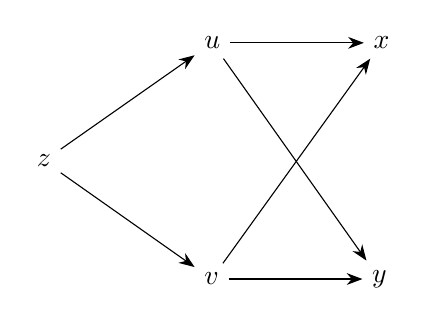
\begin{tikzpicture}[node distance=11mm and 17mm,>={Stealth[length=2mm]}]
\node (z) {$z$};
\node (u) [above right=of z] {$u$};
\node (v) [below right=of z] {$v$};
\node (x) [right=of u] {$x$};
\node (y) [right=of v] {$y$};
\draw[->] (z)--(u); \draw[->] (z)--(v);
\draw[->] (u)--(x); \draw[->] (u)--(y);
\draw[->] (v)--(x); \draw[->] (v)--(y);
\end{tikzpicture}
\end{center}

此外，做题时常出现忘了某变量其实是自变量的函数，从而求导时忘记对其求偏导的情况。建议做提前就把计算图列好，避免这种情况。

\textbf{3. 反函数求导}
\[
\frac{\dd x}{\dd y}=\frac{1}{\dd y/\dd x}.
\]

\textbf{4. 隐函数（组）求（偏）导}

\begin{center}
\begin{tabularx}{\textwidth}{>{\bfseries}p{2.5cm}XXX}
\toprule
 & 一元数量值函数 & 多元数量值函数 & 多元向量值函数 \\
\midrule
隐函数（组）求导 &
$\dfrac{\dd y}{\dd x}=-\dfrac{F_x}{F_y}$ &
$\nabla_{\bm x}y=-\dfrac{1}{F_y}\nabla_{\bm x}F$ &
$\bm J_{\bm x}\bm y=-(\bm J_{\bm y}\bm F)^{-1}\bm J_{\bm x}\bm F$ \\
 & &
$\dfrac{\partial y}{\partial x_i}=-\dfrac{F_{x_i}}{F_y}$ &
$\dfrac{\partial y_j}{\partial x_i}=-\dfrac{F_{x_i}}{F_{y_j}}$ \\
\bottomrule
\end{tabularx}
\end{center}

容易注意到存在（偏）导数的前提是 $F_y\neq0$ 或 $\bm J_{\bm y}\bm F$ 可逆。

有解析式的隐函数（组）求（偏）导均可以简化为求 $F(\bm x,\bm y)=0$ 的全微分方程 $\mathrm DF=0$，再将因变量微分用自变量微分表示，即可得到所求（偏）导数。此处不赘述。其本质是链式法则与线性方程求解。

\subsubsection{具体定理}

\textbf{1. 微分中值定理}

\textbf{（1）Fermat 定理}
\[
\left.
\begin{array}{l}
f\text{ 在 }x_0\text{ 处取极值},\\
f'(x_0)\text{ 存在}
\end{array}
\right\}
\Longrightarrow f'(x_0)=0.
\]

\textbf{（2）Rolle 定理}
\[
\left.
\begin{array}{l}
f\in C[a,b],\\
f\in D(a,b),\\
f(a)=f(b)
\end{array}
\right\}
\Longrightarrow
\exists\xi\in(a,b),\ \text{s.t. }f'(\xi)=0.
\]

\textbf{（3）Lagrange 定理}
\[
\left.
\begin{array}{l}
f\in C[a,b],\\
f\in D(a,b)
\end{array}
\right\}
\Longrightarrow
\exists\xi\in(a,b),\ \text{s.t. }
f(b)-f(a)=f'(\xi)(b-a).
\]

\textbf{（4）Cauchy 定理}
\[
\left.
\begin{array}{l}
f,g\in C[a,b],\\
f,g\in D(a,b),\\
\forall x\in(a,b),\ g'(x)\neq0
\end{array}
\right\}
\Longrightarrow
\exists\xi\in(a,b),\ \text{s.t. }
\frac{f(b)-f(a)}{g(b)-g(a)}=\frac{f'(\xi)}{g'(\xi)}.
\]

\textbf{2. Taylor 公式}

一元数量值函数 Taylor 公式：
\[
\begin{aligned}
f(x)={}&f(x_0)+f'(x_0)(x-x_0)+\frac{1}{2!}f''(x_0)(x-x_0)^2+\cdots\\
&+\frac{1}{n!}f^{(n)}(x_0)(x-x_0)^n+o\!\left((x-x_0)^n\right).
\end{aligned}
\]

多元数量值函数二阶 Taylor 公式：
\[
f(\bm x)=f(\bm x_0)+\inner{\nabla f(\bm x_0)}{\Delta\bm x}
+\frac{1}{2!}(\Delta\bm x)^T\bm H_f(\bm x_0)\Delta\bm x
+o\!\left(\norm{\Delta\bm x}^2\right).
\]

\textbf{3. L'H\^{o}pital 定理}
\[
\left.
\begin{array}{l}
\displaystyle\lim_{x\to x_0^+}f(x)=\lim_{x\to x_0^+}g(x)=0\text{ 或 }\infty,\\
f,g\in D(x_0,x_0+\delta),\\
\forall x\in(x_0,x_0+\delta),\ g'(x)\neq0,\\
\displaystyle\lim_{x\to x_0^+}\frac{f'(x)}{g'(x)}=a
\end{array}
\right\}
\Longrightarrow
\lim_{x\to x_0^+}\frac{f(x)}{g(x)}
=\lim_{x\to x_0^+}\frac{f'(x)}{g'(x)}=a.
\]

\subsection{应用}

\subsubsection{数量值函数性质研究}

\textbf{1. 单调性、极值与最值}

\textbf{（1）单调性}

\begin{center}
\begin{tabularx}{0.88\textwidth}{XX}
\toprule
单调增加：$f'(x)\geq0$ & 严格单调增加：$f'(x)>0$ \\
单调减少：$f'(x)\leq0$ & 严格单调减少：$f'(x)<0$ \\
\bottomrule
\end{tabularx}
\end{center}

\textbf{（2）无约束极值}

\begin{center}
\begin{tabularx}{\textwidth}{>{\bfseries}p{2.5cm}XX}
\toprule
 & 一元数量值函数 & 多元数量值函数 \\
\midrule
驻点 & $f'(x)=0$ & $\nabla f=0$ \\
极小值点 & $f'(x)=0$ 且 $f''(x)>0$ & $\nabla f=0$ 且 $\bm H_f\succ0$ \\
极大值点 & $f'(x)=0$ 且 $f''(x)<0$ & $\nabla f=0$ 且 $\bm H_f\prec0$ \\
鞍点 & / & $\nabla f=0$ 且 $\bm H_f$ 不定 \\
\bottomrule
\end{tabularx}
\end{center}

注：极值点判断是充分不必要条件，若无法判断正定、负定或不定时需具体情况具体分析；此外要注意间断点也可能出现极值！

\textbf{（3）有约束极值——Lagrange 乘数法}

函数 $f(\bm x)$ 与约束条件 $\varphi(\bm x)=0$ 可构建 Lagrange 函数
\[
L(\bm x,\lambda)=f(\bm x)+\lambda\varphi(\bm x).
\]
使 $\nabla L=0$，求得 $\bm x_0$ 即 $f(\bm x)$ 的有约束驻点，再结合具体情况判断该驻点是否为极值点。

\textbf{（4）最值}

无约束极值 $+$ 边界条件有约束极值 $+$ 间断点，不多赘述。

\textbf{2. 凹凸性与拐点}

\begin{center}
\begin{tabularx}{\textwidth}{>{\bfseries}p{2.5cm}XX}
\toprule
 & 一元数量值函数 & 多元数量值函数 \\
\midrule
凹 & $f''(x)\geq0$ & $\bm H_f\succeq0$ \\
凸 & $f''(x)\leq0$ & $\bm H_f\preceq0$ \\
特殊点 & 拐点：$f''(x)=0$ & 鞍点：$\bm H_f$ 不定 \\
\bottomrule
\end{tabularx}
\end{center}

严格凹凸去掉等号即可。注：此处凹凸函数仅以直观形象定义。具体凹凸函数定义各家不同，依据其定义即可。

\subsubsection{解析几何应用}

\textbf{1. 切向量与法向量}

$n$ 维 Euclid 空间中的连续超曲面，在任意点处均满足：

\begin{itemize}
  \item 能够张成 $\nabla f$ 的极大线性无关组中每个分量均是该点的法向量；
  \item 在所求点以 $\dd\bm x$ 为未知量列方程
  \[
  \inner{\nabla f}{\dd\bm x}=0,
  \]
  所得基础解系中的每个向量均是该点的切向量。
\end{itemize}

\textbf{2. Frenet 标架}

\begin{center}
\begin{tabularx}{\textwidth}{>{\bfseries}p{2.1cm}XXX}
\toprule
向量名称 & 切向量 & 主法向量 & 从法向量 \\
\midrule
定义 &
$\bm T(t)=\dfrac{\bm r'(t)}{\norm{\bm r'(t)}}$ &
$\bm N(t)=\dfrac{\bm T'(t)}{\norm{\bm T'(t)}}$ &
$\bm B(t)=\bm T(t)\times\bm N(t)=\dfrac{\bm r'(t)\times\bm r''(t)}{\norm{\bm r'(t)\times\bm r''(t)}}$ \\
意义 & 曲线前进方向 & 曲线弯曲方向 & 曲线偏离切平面方向 \\
对应直线 & 切线 & 主法线 & 从法线 \\
对应特征平面 & 法平面 $\inner{\bm r-\bm r_0}{\bm T}=0$ &
从切平面 $\inner{\bm r-\bm r_0}{\bm N}=0$ &
密切平面 $\inner{\bm r-\bm r_0}{\bm B}=0$ \\
\bottomrule
\end{tabularx}
\end{center}

\textbf{3. 曲率与挠率}

\begin{center}
\begin{tabularx}{\textwidth}{>{\bfseries}p{2.2cm}XX}
\toprule
 & 曲率 & 挠率 \\
\midrule
定义 & $\kappa=\left\lVert\dfrac{\dd\bm T}{\dd s}\right\rVert$ & $\tau=-\bm B'(s)\cdot\bm N(s)$ \\
自然坐标 & $\kappa=\norm{\bm r''(s)}$ & $\tau=\dfrac{[\bm r'(s),\bm r''(s),\bm r'''(s)]}{\norm{\bm r''(s)}^2}$ \\
参数坐标 & $\kappa=\dfrac{\norm{\bm r'(t)\times\bm r''(t)}}{\norm{\bm r'(t)}^3}$ & $\tau=\dfrac{[\bm r'(t),\bm r''(t),\bm r'''(t)]}{\norm{\bm r'(t)\times\bm r''(t)}^2}$ \\
直角坐标 & $\kappa=\dfrac{|y''|}{[1+(y')^2]^{3/2}}$ & $\kappa=\dfrac{|\dot x\ddot y-\ddot x\dot y|}{(\dot x^2+\dot y^2)^{3/2}}$ \\
\bottomrule
\end{tabularx}
\end{center}

此外曲率半径
\[
\rho=\frac{1}{\kappa}.
\]

\section{积分学}

\subsection{概念}

\subsubsection{不定积分}

重要提示：不定积分要加 $C$！

\subsubsection{数量值函数积分}

\textbf{1. 性质}

\textbf{线性}
\[
\int_{\Omega}\left[C_1f(M)\pm C_2g(M)\right]\dd\Omega
=C_1\int_{\Omega}f(M)\dd\Omega
\pm C_2\int_{\Omega}g(M)\dd\Omega.
\]

\textbf{积分域可加性}
\[
\int_{\Omega}f(M)\dd\Omega
=\int_{\Omega_1}f(M)\dd\Omega
+\int_{\Omega_2}f(M)\dd\Omega,
\qquad \Omega=\Omega_1\cup\Omega_2.
\]

\textbf{积分不等式}

若 $f(M)\leq g(M)$，$\forall M\in\Omega$，则
\[
\int_{\Omega}f(M)\dd\Omega\leq\int_{\Omega}g(M)\dd\Omega.
\]
并且
\[
\left|\int_{\Omega}f(M)\dd\Omega\right|
\leq\int_{\Omega}|f(M)|\dd\Omega.
\]
若 $l\leq f(M)\leq L$，$\forall M\in\Omega$，则
\[
l|\Omega|\leq\int_{\Omega}f(M)\dd\Omega\leq L|\Omega|.
\]

\textbf{轴对称性}

定义较繁琐，记住关于坐标轴“奇零偶倍”即可。

\textbf{轮换对称性}

定义较繁琐。简单讲，若交换 $x,y,z$ 位置，积分域与函数都不变，则可以用轮换对称。

\textbf{2. 定积分与重积分}

\begin{center}
\begin{tabularx}{\textwidth}{>{\bfseries}p{2.4cm}XXX}
\toprule
体积微元 & 定积分 & 二重积分 & 三重积分 \\
\midrule
直角坐标 & 就正常积咯 & $\dd\sigma=\dd x\dd y$ & $\dd V=\dd x\dd y\dd z$ \\
极坐标/柱坐标 & / & $\dd\sigma=\rho\dd\rho\dd\theta$ & $\dd V=\rho\dd\rho\dd\theta\dd z$ \\
球坐标 & / & / & $\dd V=r^2\sin\varphi\dd r\dd\varphi\dd\theta$ \\
曲面坐标 & / & $\dd\sigma=\left|\dfrac{\partial(x,y)}{\partial(u,v)}\right|\dd u\dd v$ & $\dd V=\left|\dfrac{\partial(x,y,z)}{\partial(u,v,w)}\right|\dd u\dd v\dd w$ \\
\bottomrule
\end{tabularx}
\end{center}

二重积分域为圆域或与圆相关的积分域时多用极坐标。要注意圆心在原点时 $0\leq\rho\leq R$，圆过原点时 $0\leq\rho\leq2R\cos\theta$，$\rho$ 范围不同。

三重积分域为旋转体时多用柱坐标，且可以将原积分改写为
\[
\int_a^b f(x,y,z)S(z)\dd z.
\]

三重积分域为球域或与球相关的积分域时多用球坐标。要注意球心在原点时 $0\leq r\leq R$，球过原点时 $0\leq r\leq2R\cos\varphi$，$r$ 范围不同。

此外，柱坐标旋转轴与球坐标极轴的选取不唯一。可以依具体函数与积分域选择 $x$ 轴或 $y$ 轴作为旋转轴或极轴。如积分域由 $y=x^2+z^2$ 与 $y=1$ 所围区域，就适合以 $y$ 轴作为旋转轴取柱坐标积分。

\textbf{3. 多次积分换序}

法一：作图法。通过各积分上下限确定积分范围，作出图后选择适宜的积分方式。（较推荐）

法二：反函数法。求得积分上下限反函数后代入即可。但此法会产生正负不同等问题，建议还是辅助作图观察。

\textbf{4. 反常积分}

\textbf{（1）含参积分}

一元数量值函数：
\[
\frac{\dd}{\dd x}\int_{\phi(x)}^{\varphi(x)}f(t)\dd t
=f(\varphi(x))\varphi'(x)-f(\phi(x))\phi'(x).
\]

二元数量值函数：
\[
\begin{aligned}
\frac{\partial}{\partial y}
\int_{x_1(y)}^{x_2(y)}\int_{y_1(x)}^{y_2(x)}f(x,y)\dd y\dd x
={}&\int_{x_1(y)}^{x_2(y)}\frac{\partial f(x,y)}{\partial y}\dd x\\
&+f(x_2(y),y)x_2'(y)-f(x_1(y),y)x_1'(y).
\end{aligned}
\]

\textbf{（2）反常积分判敛准则}

\begin{method}[判断反常函数敛散性]
第一步：判断是无穷积分还是瑕积分，注意观察 $x$ 的趋近方向。

第二步：求出函数的等价无穷小。对于无穷积分，若
\[
f(x)\sim\frac1{x^p},\qquad p>1,
\]
则收敛；对于瑕积分，若
\[
f(x)\sim\frac1{x^p},\qquad0<p<1,
\]
则收敛。

$f(x)\sim1/x$ 任何情况下都不收敛！
\end{method}

\subsubsection{第一型曲线曲面积分}

核心特征：数量值函数与向量模的乘积。

特殊性质：代入性。

核心处理方法：求出切向量或法向量的模并代入，即将第一型曲线曲面积分转化为定积分或重积分。

\begin{center}
\begin{tabularx}{\textwidth}{>{\bfseries}p{2.1cm}XX}
\toprule
 & 第一型曲线积分 & 第一型曲面积分 \\
\midrule
本质 & $\displaystyle\int_C f(s)\dd s=\int_C f(t)\norm{\bm r'(t)}\dd t$ & $\displaystyle\iint_S f(S)\dd S=\iint_S f(u,v)\norm{\bm r_u\times\bm r_v}\dd u\dd v$ \\
参数方程 & $\dd s=\sqrt{[x'(t)]^2+[y'(t)]^2}\dd t$ & $\dd S=\norm{\bm r_u\times\bm r_v}\dd u\dd v$ \\
直角方程 & $\dd s=\sqrt{1+[y'(x)]^2}\dd x$ & $\dd S=\sqrt{1+z_x^2+z_y^2}\dd x\dd y$ \\
隐式曲面 & / & $\displaystyle\dd S=\frac{\sqrt{F_x^2+F_y^2+F_z^2}}{|F_z|}\dd x\dd y$ \\
极坐标方程 & $\dd s=\sqrt{\rho^2(\theta)+[\rho'(\theta)]^2}\dd\theta$ & 圆柱面：$\dd S=\rho\dd\theta\dd z$ \\
球面 & / & $\dd S=R^2\sin\varphi\dd\theta\dd\varphi$ \\
\bottomrule
\end{tabularx}
\end{center}

积分转换关系一图览：
\[
\boxed{\text{第二型曲线积分}}
\xleftrightarrow[\text{单位切向量}]{\text{向量微元}}
\boxed{\text{第一型曲线积分}}
\longleftrightarrow
\boxed{\text{定积分}},
\]
\[
\boxed{\text{第二型曲面积分}}
\xleftrightarrow[\text{单位法向量}]{\text{向量微元}}
\boxed{\text{第一型曲面积分}}
\longleftrightarrow
\boxed{\text{重积分}}.
\]

第一型曲面积分不一定要投影到 $xOy$ 面上，以方便计算为准。对圆柱面与球面积分时可采用简便的极坐标微元。此外，当球面坐标形如
\[
\iint_S\frac{f(x,y)}{z}\dd S
\]
时，直接选用微元代换
\[
\dd S=\frac{R}{|z|}\dd x\dd y.
\]
分母是 $x,y$ 时同理。

求球面的截面积小技巧：
\[
S=2\pi Rh,
\]
其中 $h$ 为两截面间距离。

\subsubsection{第二型曲线曲面积分}

核心特征：向量值函数与向量微元的内积。

特殊性质：代入性。

注意事项：注意积分路径方向！此外要复习空间曲线切向量与曲面法向量求法。一般规定曲线积分左侧为积分域方向为正向，曲面积分法向量与坐标轴交角小于 $\pi/2$ 为正向，但以题目规定为准。

核心处理方法：将第二型曲线曲面积分转换为第一型曲线曲面积分。其一，将向量微元处理为切向量或法向量乘数量微元；其二，利用 Stokes 公式转换。

\begin{center}
\begin{tabularx}{\textwidth}{>{\bfseries}p{2.1cm}XX}
\toprule
 & 第二型曲线积分 & 第二型曲面积分 \\
\midrule
本质 & $\displaystyle\int_C\bm A(\bm s)\cdot\dd\bm s=\int_C\bm A(t)\cdot\bm r'(t)\dd t$ & $\displaystyle\iint_S\bm A(\bm S)\cdot\dd\bm S=\iint_S\bm A\cdot\bm n\dd S$ \\
参数方程 & $\dd\bm s=(x'(t),y'(t))\dd t$ & $\dd\bm S=(\bm r_u\times\bm r_v)\dd u\dd v$ \\
直角方程 & $\dd\bm s=(1,y'(x))\dd x$ & $\displaystyle\dd\bm S=\left(\frac{\cos\alpha}{\cos\gamma},\frac{\cos\beta}{\cos\gamma},1\right)\dd x\dd y$ \\
\bottomrule
\end{tabularx}
\end{center}

\subsection{定理}

\textbf{1. 微积分基本定理}

第一基本定理：
\[
\frac{\dd}{\dd x}\int_a^x f(t)\dd t=f(x).
\]

第二基本定理：若 $F$ 是 $f$ 的原函数，则 $F+C$ 也是 $f$ 的原函数。

重要提示：不定积分要加 $C$！

\textbf{2. 积分技巧}

重要提示：定积分换元必换限！

\textbf{（1）换元法}

换元法 I：令 $u=\varphi(x)$，则
\[
\int f[\varphi(x)]\varphi'(x)\dd x=\int f(u)\dd u.
\]

换元法 II：令 $x=\varphi(t)$，则
\[
\int f(x)\dd x=\int f[\varphi(t)]\varphi'(t)\dd t.
\]

使用上述两种换元法，要熟悉常见初等函数与其导数的关系。

三角换元法常用于含平方差或平方和的被积式中，一般代换如下：
\[
\begin{array}{lll}
\sqrt{a^2-x^2}:&x=a\sin t,&\dd x=a\cos t\dd t,\\
\sqrt{a^2+x^2}:&x=a\tan t,&\dd x=a\sec^2t\dd t,\\
\sqrt{x^2-a^2}:&x=a\sec t,&\dd x=a\sec t\tan t\dd t.
\end{array}
\]

根式代换法：作代换
\[
t^2=ax+b,\qquad\dd x=\frac{2t}{a}\dd t.
\]
此法适用于带根式的积分。

倒代换法：作代换
\[
t=\frac1x,\qquad\dd x=-\frac1{t^2}\dd t.
\]
观察不难得出，当分子分母次数相差 $2$ 以上时该法较为好用。

配方法：将含有 $ax^2+bx+c$ 的部分配方，随后用三角换元法。

\textbf{（2）分部法}
\[
\int u\dd v=uv-\int v\dd u.
\]
顺序：反对函三指。当被积式中含有两种函数的乘积时，一般采用分部法。

\textbf{（3）消元法}

消元法是特殊的分部法。可以记作
\[
\int[\varphi(x)+\varphi'(x)]e^x\dd x=e^x\varphi(x)+C.
\]
例如
\[
\int\left(\ln x+\frac1x\right)e^x\dd x=e^x\ln x+C.
\]

\textbf{（4）循环法}

循环法是分部法的延伸。因为如 $e^x$、$\sin x$、$\cos x$ 等函数的导数或多次导数与原函数相同，可借此解方程求得原积分值。常见积分：
\[
\int e^{ax}\sin bx\dd x
=\frac{e^{ax}}{a^2+b^2}(a\sin bx-b\cos bx)+C,
\]
\[
\int e^{ax}\cos bx\dd x
=\frac{e^{ax}}{a^2+b^2}(a\cos bx+b\sin bx)+C.
\]

\textbf{（5）配对法}

配对法是循环法的延伸。原积分不好求，则选择另一个函数与之配凑，得到关于积分的方程组，顺势求解。

例如
\[
I=\int\frac{1}{1+x^3}\dd x,
\qquad
J=\int\frac{x}{1+x^3}\dd x,
\]
可通过 $I+J$ 与 $I-J$ 分别拆分为容易积分的有理式。

\textbf{（6）配次法}

对于积分
\[
\int\frac{1}{x(x^n\pm1)}\dd x,
\]
先在分子分母同时乘以 $x^{n-1}$，得到
\[
\int\frac{1}{x(x^n\pm1)}\dd x
=\int\frac{x^{n-1}}{x^n(x^n\pm1)}\dd x,
\]
即可拆开分别积分。

\textbf{（7）公式法}
\[
\int_a^b f(x)\dd x
=\int_0^{(b-a)/2}\left[
f\left(\frac{a+b}{2}-x\right)
+f\left(\frac{a+b}{2}+x\right)
\right]\dd x,
\]
\[
\int_a^b f(x)\dd x
=\frac12\int_a^b[f(x)+f(a+b-x)]\dd x.
\]

\textbf{（8）有理积分}

有理积分必可积。

\textbf{（9）三角积分}

由半角公式，作代换 $t=\tan(x/2)$：
\[
\sin x=\frac{2t}{1+t^2},\qquad
\cos x=\frac{1-t^2}{1+t^2},\qquad
\dd x=\frac{2}{1+t^2}\dd t.
\]
则三角积分化为有理积分，必可积。此公式又称万能公式。但此法过于繁琐，一般不用，可用下面的方法简单判断：

\begin{enumerate}
  \item 若 $\sin$ 为奇次、$\cos$ 为偶次，则取 $\dd(\cos x)$ 或 $\dd(\sec x)$；
  \item 若 $\sin$ 为偶次、$\cos$ 为奇次，则取 $\dd(\sin x)$ 或 $\dd(\csc x)$；
  \item 若 $\sin$、$\cos$ 同次，则取 $\dd(\tan x)$ 或 $\dd(\cot x)$。
\end{enumerate}

此外，还要善于利用降次公式、和差倍半、和差化积、三角恒等式、Wallis 公式等三角公式。

Wallis 公式：
\[
\int_0^{\pi/2}\sin^n x\dd x=
\begin{cases}
\dfrac{(n-1)(n-3)\cdots3\cdot1}{n(n-2)\cdots4\cdot2}\dfrac{\pi}{2},&n\text{ 为偶数},\\[6pt]
\dfrac{(n-1)(n-3)\cdots4\cdot2}{n(n-2)\cdots3\cdot1},&n\text{ 为奇数}.
\end{cases}
\]

\textbf{3. 积分中值定理}
\[
f\in C(\Omega)\Longrightarrow
\exists P\in\Omega,\ \text{s.t. }
\int_{\Omega}f(M)\dd\Omega=f(P)|\Omega|.
\]

和积分有关的证明题基本都会用到积分中值定理。套路不明显，不赘述。

有一类计算题会用到积分中值定理，一般形如
\[
\lim_{t\to0^+}\frac{1}{t^2}\iint_{S(t)}f(M)\dd\sigma,
\]
其中 $t\to0^+$ 时圆域 $S(t)$ 收敛于一个点。一般做法是运用积分中值定理：
\[
\lim_{t\to0^+}\frac{1}{\pi t^2}\iint_{S(t)}f(M)\dd\sigma,
\]
极限值为 $f$ 在圆心处的值。

\subsection{应用}

\subsubsection{几何应用}

若求弧长，一般用第一型曲线积分；若求曲面面积，一般用第一型曲面积分；若求体积，一般用第二型曲面积分。

\subsubsection{物理应用}

\begin{enumerate}
  \item 形心：
  \[
  \bm r_C=\frac{\displaystyle\int_V\bm r\dd V}{\displaystyle\int_V\dd V};
  \]
  \item 质心：
  \[
  \bm r_{MC}=\frac{\displaystyle\int_V\mu\bm r\dd V}{\displaystyle\int_V\mu\dd V};
  \]
  \item 转动惯量：
  \[
  J=\int_V\mu r^2\dd V.
  \]
\end{enumerate}

\section{常微分方程}

\subsection{一阶常微分方程}

\textbf{1. 可分离变量的一阶常微分方程}

若方程形如
\[
\frac{\dd y}{\dd x}=f(x)g(y),
\]
则由下式确定的隐函数为该方程的解：
\[
\int\frac{\dd y}{g(y)}=\int f(x)\dd x+C.
\]

\textbf{2. 一阶线性微分方程}

若方程形如
\[
\frac{\dd y}{\dd x}+P(x)y=Q(x),
\]
则下式即为该方程的解：
\[
y=e^{-\int P(x)\dd x}
\left[\int Q(x)e^{\int P(x)\dd x}\dd x+C\right].
\]

\textbf{3. 可得到一阶常微分方程的代换法}

\textbf{（1）齐次微分方程}

若方程形如
\[
\frac{\dd y}{\dd x}=f\!\left(\frac yx\right),
\]
作代换
\[
u=\frac yx,
\qquad
\frac{\dd y}{\dd x}=u+x\frac{\dd u}{\dd x},
\]
得到可分离变量方程
\[
u+x\frac{\dd u}{\dd x}=f(u),
\]
即可求解。

\textbf{（2）Bernoulli 方程}

若方程形如
\[
\frac{\dd y}{\dd x}+P(x)y=Q(x)y^\alpha,
\]
两边除以 $y^\alpha$，作代换
\[
u=y^{1-\alpha},
\qquad
\frac{\dd u}{\dd x}=(1-\alpha)y^{-\alpha}\frac{\dd y}{\dd x},
\]
得到一阶线性微分方程
\[
\frac{\dd u}{\dd x}+(1-\alpha)P(x)u=(1-\alpha)Q(x),
\]
即可求解。

\textbf{4. 可降为一阶方程的高阶常微分方程}

\textbf{（1）$y^{(n)}=f(x)$}

过于简单，不论。

\textbf{（2）$y''=f(x,y')$}

作代换
\[
p=\frac{\dd y}{\dd x},
\]
即可得到一阶常微分方程
\[
\frac{\dd p}{\dd x}=f(x,p).
\]
原方程通解为
\[
y=\int F(x,C_1)\dd x+C_2.
\]

\textbf{（3）$y''=f(y,y')$}

作代换
\[
p=\frac{\dd y}{\dd x},
\qquad
y''=\frac{\dd p}{\dd x}
=\frac{\dd p}{\dd y}\frac{\dd y}{\dd x}
=p\frac{\dd p}{\dd y},
\]
即可得到一阶常微分方程并求解。

\subsection{二阶常系数齐次常微分方程}

\textbf{1. 通解}

写出特征方程
\[
\lambda^2+a_1\lambda+a_2=0,
\]
并求得特征根，根据下表写出通解。

\begin{center}
\begin{tabularx}{\textwidth}{>{\bfseries}p{3cm}p{3.6cm}X}
\toprule
特征根 & 条件 & 通解 \\
\midrule
两个不同实根 & $\lambda_1\neq\lambda_2$ & $x=C_1e^{\lambda_1t}+C_2e^{\lambda_2t}$ \\
两个相同实根 & $\lambda_1=\lambda_2$ & $x=(C_1t+C_2)e^{\lambda_1t}$ \\
共轭复根 & $\lambda_{1,2}=\alpha\pm i\beta$ & $x=e^{\alpha t}(C_1\cos\beta t+C_2\sin\beta t)$ \\
\bottomrule
\end{tabularx}
\end{center}

\textbf{2. 特解}

对于非齐次常微分方程
\[
x''+a_1x'+a_2x=F(t),
\]
需要根据 $F(t)$ 的形式确定特解形式，代回原方程求得特解。

若
\[
F(t)=\varphi(t)e^{\mu t},
\]
其中 $\mu$ 为 $k$ 重特征根，则取
\[
x^*=t^ke^{\mu t}Z(t).
\]

若
\[
F(t)=\varphi(t)e^{\mu t}\cos\nu t
\quad\text{或}\quad
F(t)=\varphi(t)e^{\mu t}\sin\nu t,
\]
其中 $\mu\pm i\nu$ 为 $k$ 重特征根，则取
\[
x^*=t^ke^{\mu t}[Z_1(t)\cos\nu t+Z_2(t)\sin\nu t].
\]
其中 $Z(t)$、$Z_1(t)$ 和 $Z_2(t)$ 均为与 $\varphi(t)$ 次数相等的多项式。

\section{向量分析与场论}

\subsection{概念}

定义 Nabla 算子
\[
\nabla=\left(\frac{\partial}{\partial x_1},
\frac{\partial}{\partial x_2},\ldots,
\frac{\partial}{\partial x_n}\right),
\]
Laplace 算子
\[
\Delta=\nabla^2=\sum_{i=1}^{n}\frac{\partial^2}{\partial x_i^2}.
\]

\textbf{1. 环量与通量}

\textbf{（1）环量}

作闭合曲线 $C$，定义环量
\[
\Gamma=\oint_C\bm A\cdot\dd\bm s.
\]
保证法向量方向不变的前提下，曲线 $C$ 以任意方式缩小为点 $M$ 时，若极限
\[
\lim_{\Delta S\to0}\frac{\Delta\Gamma}{\Delta S}
\]
存在，则定义环量密度
\[
\frac{\dd\Gamma}{\dd S}\bm n.
\]

\textbf{（2）通量}

作闭合曲面 $S$，定义通量
\[
\Phi=\oiint_S\bm A\cdot\dd\bm S.
\]
若 $\Phi=0$，说明曲面内部无源或汇，否则有源或汇。

曲面 $S$ 以任意方式缩小为点 $M$ 时，若极限
\[
\lim_{\Delta V\to0}\frac{\Delta\Phi}{\Delta V}
\]
存在，则定义通量密度（即散度）
\[
\operatorname{div}\bm A=\nabla\cdot\bm A
=\frac{\dd\Phi}{\dd V}.
\]

\textbf{2. 梯度、旋度与散度}

\textbf{（1）梯度}

梯度是向量值，指示数量场在某点上升最快的速度和方向，用 $\nabla f$ 表示。

线性：
\[
\nabla(C_1u+C_2v)=C_1\nabla u+C_2\nabla v.
\]
运算性质：
\[
\nabla(uv)=u\nabla v+v\nabla u,
\qquad
\nabla\left(\frac uv\right)=\frac{v\nabla u-u\nabla v}{v^2}.
\]
复合法则：
\[
\nabla f(u)=f'(u)\nabla u.
\]

\textbf{（2）旋度}

旋度是向量值，指示向量场在某点的旋转强度与方向，用 $\nabla\times\bm A$ 表示。数量上等于该点环量密度的最大值，方向即环量密度最大方向。

线性：
\[
\nabla\times(C_1\bm A\pm C_2\bm B)
=C_1\nabla\times\bm A\pm C_2\nabla\times\bm B.
\]
运算性质：
\[
\nabla\times(u\bm A)=u\nabla\times\bm A+\nabla u\times\bm A.
\]

\textbf{（3）散度}

散度是数量值，指示向量场在某点发散或汇聚的强度，用 $\nabla\cdot\bm A$ 表示。散度即通量密度。

线性：
\[
\nabla\cdot(C_1\bm A\pm C_2\bm B)
=C_1\nabla\cdot\bm A\pm C_2\nabla\cdot\bm B.
\]
运算性质：
\[
\nabla\cdot(u\bm A)=u\nabla\cdot\bm A+\nabla u\cdot\bm A.
\]

\textbf{（4）其他计算公式}

梯度场无旋：
\[
\nabla\times(\nabla u)=\bm0.
\]
旋度场无源：
\[
\nabla\cdot(\nabla\times\bm A)=0.
\]
向量积散度公式：
\[
\nabla\cdot(\bm A\times\bm B)
=\bm B\cdot(\nabla\times\bm A)-\bm A\cdot(\nabla\times\bm B).
\]
梯度场散度公式：
\[
\nabla\cdot(\nabla u)=\nabla^2u.
\]
旋度场旋度公式：
\[
\nabla\times(\nabla\times\bm A)
=\nabla(\nabla\cdot\bm A)-\nabla^2\bm A.
\]

\textbf{3. 特殊向量场}

\textbf{（1）无旋场}

单连通区域内，无旋场、有势场、保守场等价。设 $\bm A\in C^1(G)$，$G\subset\R^3$：
\[
\begin{array}{ll}
\text{无旋场：}&\nabla\times\bm A=\bm0,\\
\text{有势场：}&\exists u,\ \text{s.t. }\bm A=\nabla u,\\
\text{保守场：}&\displaystyle\oint_C\bm A\cdot\dd\bm s=0.
\end{array}
\]

积分与路径无关等价于保守场、旋度为 $0$，即等价于 $\nabla\times\bm A=\bm0$。

\textbf{（2）无源场}

单连通区域内，无源场、向量有势场、保守场等价：
\[
\begin{array}{ll}
\text{无源场：}&\nabla\cdot\bm A=0,\\
\text{向量有势场：}&\exists\bm B,\ \text{s.t. }\bm A=\nabla\times\bm B,\\
\text{保守场：}&\displaystyle\oiint_S\bm A\cdot\dd\bm S=0.
\end{array}
\]

\textbf{（3）调和场}

调和场势函数满足 Laplace 方程
\[
\nabla^2u=0,
\]
即
\[
\frac{\partial^2u}{\partial x^2}
+\frac{\partial^2u}{\partial y^2}
+\frac{\partial^2u}{\partial z^2}=0.
\]

\subsection{定理}

\textbf{0. Newton--Leibniz 公式}
\[
\int_a^b f'(x)\dd x=f(b)-f(a).
\]

\textbf{1. Green 公式}

设平面有界闭域 $\sigma$ 由分段光滑的简单闭曲线围成，$\sigma$ 的边界曲线记为 $C$，函数 $P,Q\in C^1(\sigma)$，则
\[
\iint_{\sigma}\left(\frac{\partial Q}{\partial x}-\frac{\partial P}{\partial y}\right)\dd x\dd y
=\oint_{C^+}P\dd x+Q\dd y.
\]

\textbf{2. Stokes 公式}
\[
\iint_S\left(\frac{\partial R}{\partial y}-\frac{\partial Q}{\partial z}\right)\dd y\wedge\dd z
+\left(\frac{\partial P}{\partial z}-\frac{\partial R}{\partial x}\right)\dd z\wedge\dd x
+\left(\frac{\partial Q}{\partial x}-\frac{\partial P}{\partial y}\right)\dd x\wedge\dd y
=\oint_{C^+}P\dd x+Q\dd y+R\dd z.
\]

几何意义为旋度对面积的积分等于原函数在外曲线上的积分，即向量形式
\[
\iint_S(\nabla\times\bm A)\cdot\dd\bm S
=\oint_{C^+}\bm A\cdot\dd\bm s.
\]

\textbf{3. Gauss 公式}

设空间有界闭域 $V$ 由分段光滑的简单闭曲面 $S$ 围成，向量函数 $\bm A=(P,Q,R)\in C^1(V)$，则
\[
\iiint_V\left(\frac{\partial P}{\partial x}
+\frac{\partial Q}{\partial y}
+\frac{\partial R}{\partial z}\right)\dd V
=\oiint_{S^+}P\dd y\wedge\dd z
+Q\dd z\wedge\dd x
+R\dd x\wedge\dd y.
\]

几何意义为散度对体积的积分等于原函数在外表面上的积分，即向量形式
\[
\iiint_V\nabla\cdot\bm A\dd V
=\oiint_{S^+}\bm A\cdot\dd\bm S.
\]

上三式可以统一于如下公式，受限于知识水平不作进一步介绍。

\textbf{4. 广义 Stokes 公式}
\[
\int_{\Omega}\dd\omega=\int_{\partial\Omega}\omega.
\]

\begin{method}[广义 Stokes 公式求第二型曲线曲面积分]
广义 Stokes 公式是解题一把好手。使用广义 Stokes 公式解题时应注意以下三点：

\begin{enumerate}
  \item 原函数处处有定义，尤其是原点；
  \item 路径为正；
  \item 原函数可导。
\end{enumerate}

此外，还要注意正负与方向：曲线左侧为积分区域时为正，否则为负；曲面外侧为正，内侧为负。常用方法为右手定则。

常用方法有二：

\textbf{填补法}：将不完整的曲线或曲面补为闭合曲线或曲面，通过
\[
\int_{\Omega}\bm A\cdot\dd\bm\omega
=\int_{\Sigma^+}\bm A\cdot\dd\bm\omega
+\int_{\Sigma^-}\bm A\cdot\dd\bm\omega,
\]
即用闭合曲线或曲面积分减去添加曲线或曲面积分，得到原始路径积分。该方法通常有两种特征：

\begin{enumerate}
  \item 图形便于填补，如半圆、扇形弧，柱体侧面、锥体侧面、各种旋转体侧面；
  \item 图形补充后闭合部分散度为 $0$，即 $\nabla\cdot\bm A=0$。
\end{enumerate}

\textbf{挖空法}：用于定义域内存在间断点的情况，以原点居多。此时需用到路径变形定理。

二维表述：在无旋场中，内部包含奇点的同伦同向闭合曲线积分值相同。为将原函数表达式中形如
\[
\frac{x^2}{a^2}+\frac{y^2}{b^2}
\]
的分母部分消掉，作小椭圆
\[
\begin{cases}
x=a\varepsilon\cos\theta,\\
y=b\varepsilon\sin\theta,
\end{cases}
\]
$\varepsilon\to0$ 时，同向椭圆路径上的积分值即原积分值。常见函数如
\[
\bm A=\left(-\frac{y}{x^2+y^2},\frac{x}{x^2+y^2}\right).
\]

三维表述：在无源场内，内部包含奇点的同伦同向闭合曲面积分值相同。为将原函数表达式中形如
\[
\frac{x^2}{a^2}+\frac{y^2}{b^2}+\frac{z^2}{c^2}
\]
的分母部分消掉，作小椭球体
\[
\begin{cases}
x=a\varepsilon\sin\varphi\cos\theta,\\
y=b\varepsilon\sin\varphi\sin\theta,\\
z=c\varepsilon\cos\varphi,
\end{cases}
\]
$\varepsilon\to0$ 时，同向椭球闭合曲面上的积分值即原积分值。
\end{method}

\begin{method}[由向量函数求势函数]
主要用偏积分法。即分别对 $x$、对 $y$ 积分，将二者合并得到势函数。注意要将不定积分中的 $C$ 改为 $C(x)$、$C(y)$。
\end{method}

\section{无穷级数}

在无穷级数中我们需要处理无穷维的函数，本质上 Euclid 空间拓展到了 Hilbert 空间。但该拓展在现阶段体现不明显，故略过。

\subsection{常数项级数}

\textbf{1. 性质}

\begin{enumerate}
  \item 线性：
  \[
  \sum_{n=1}^{\infty}(C_1a_n+C_2b_n)
  =C_1\sum_{n=1}^{\infty}a_n+C_2\sum_{n=1}^{\infty}b_n.
  \]
  \item 若 $a_n\leq b_n$，则
  \[
  \sum_{n=1}^{\infty}a_n\leq\sum_{n=1}^{\infty}b_n.
  \]
  \item 任意删去、添加或改变有限项不改变级数敛散性。
  \item 设级数 $\sum_{n=1}^{\infty}a_n$ 收敛，则
  \[
  \lim_{n\to\infty}a_n=0
  \]
  （必要条件）。
  \item 级数 $\sum_{n=1}^{\infty}a_n$ 收敛的充要条件是
  \[
  \lim_{n\to\infty}R_n=0.
  \]
  \item 不带括号级数比带括号级数收敛要求更加严格。即，不带括号收敛，带括号必收敛；不带括号发散，带括号必发散。
\end{enumerate}

\textbf{2. 审敛准则}

\textbf{（1）常用收敛函数}

等比级数
\[
\sum_{n=0}^{\infty}a\alpha^n,
\]
若 $|\alpha|<1$ 则收敛，反之则发散。

$p$-级数
\[
\sum_{n=1}^{\infty}\frac1{n^p},
\]
若 $p>1$ 则收敛，反之发散。

\textbf{（2）常用发散函数}

调和级数
\[
\sum_{n=1}^{\infty}\frac1n.
\]

\textbf{（3）正项级数审敛准则}

充要条件：部分和数列有上界。

比较准则 I：设 $a_n\leq b_n$。若 $\sum b_n$ 收敛，则 $\sum a_n$ 收敛；若 $\sum a_n$ 发散，则 $\sum b_n$ 发散。（与常用收敛函数比较。）

比较准则 II：$\forall n\in\N^+$，$b_n>0$，且
\[
\lim_{n\to\infty}\frac{a_n}{b_n}=\lambda,
\qquad \lambda\in\R^+\text{、}\lambda=0\text{ 或 }\lambda=+\infty.
\]

\begin{itemize}
  \item 若 $\lambda\in\R^+$，则 $\sum a_n$ 与 $\sum b_n$ 敛散性相同；
  \item 若 $\lambda=0$ 且 $\sum b_n$ 收敛，则 $\sum a_n$ 收敛；
  \item 若 $\lambda=+\infty$ 且 $\sum b_n$ 发散，则 $\sum a_n$ 发散。
\end{itemize}

积分准则：若存在非负单调减少函数
\[
f:[1,+\infty)\to[0,+\infty),
\qquad f(n)=a_n,
\]
则级数
\[
\sum_{n=1}^{\infty}a_n
\]
与积分
\[
\int_1^{+\infty}f(x)\dd x
\]
同敛散。

D'Alembert 准则（检比法）：
\[
\lambda=\lim_{n\to\infty}\frac{a_{n+1}}{a_n}.
\]
若 $\lambda<1$，级数 $\sum a_n$ 收敛；若 $\lambda>1$，级数 $\sum a_n$ 发散。

Cauchy 准则（检根法）：
\[
\lambda=\lim_{n\to\infty}\sqrt[n]{a_n}.
\]
若 $\lambda<1$，级数 $\sum a_n$ 收敛；若 $\lambda>1$，级数 $\sum a_n$ 发散。

检根法比检比法应用广泛。能用检比法必能用检根法，反之不成立。

负项级数乘 $-1$ 后可套用正项级数审敛准则，不多叙述。

\textbf{（4）变号级数审敛准则}

Leibniz 准则：若 $\forall n\in\N^+$，$a_{n+1}<a_n$，且
\[
\lim_{n\to\infty}a_n=0,
\]
则交错级数收敛，且
\[
|S-S_n|<a_{n+1}.
\]

绝对收敛准则：若级数
\[
\sum_{n=1}^{\infty}|a_n|
\]
收敛，则级数
\[
\sum_{n=1}^{\infty}a_n
\]
收敛。

若级数 $\sum a_n$ 绝对收敛，则其重排级数 $\sum a_n'$ 也绝对收敛，且两者和相等，即 $S=S'$。

设绝对收敛级数
\[
\sum_{n=1}^{\infty}a_n=A,
\qquad
\sum_{n=1}^{\infty}b_n=B,
\]
则 Cauchy 乘积级数
\[
\sum_{n=1}^{\infty}c_n,
\qquad c_n=\sum_{s+t=n}a_sb_t
\]
也绝对收敛，且
\[
\sum_{n=1}^{\infty}c_n=AB.
\]

\begin{method}[数项级数判敛]
\begin{enumerate}
  \item 判断 $\displaystyle\lim_{n\to\infty}a_n=0$；
  \item 若级数为交错级数，使用 Leibniz 判别法；
  \item 若级数为正项级数，使用检比法或检根法。
\end{enumerate}
\end{method}

\subsection{函数项级数}

\textbf{1. 判敛准则}

Weierstrass 准则（又称 $M$ 判别准则）：如果存在一个收敛的正项级数
\[
\sum_{n=1}^{\infty}M_n,
\]
对于 $\forall n\in\N^+$ 以及 $\forall x\in D$，恒有
\[
|u_n(x)|\leq M_n,
\]
那么级数
\[
\sum_{n=1}^{\infty}u_n(x)
\]
在 $D$ 上一致收敛。

\textbf{2. 一致收敛级数性质}

\begin{enumerate}
  \item 和函数连续性：若级数函数连续，则和函数连续；
  \item 和函数可积性：若级数函数一致收敛，则和函数可积；
  \item 和函数可导性：若级数函数一致收敛，则和函数可导。
\end{enumerate}

\subsection{常用级数}

\subsubsection{幂级数}

\textbf{1. 收敛半径、收敛区间与收敛域}

D'Alembert 法（检比法）：
\[
R=\lim_{n\to\infty}\left|\frac{a_n}{a_{n+1}}\right|.
\]

Cauchy 法（检根法）：
\[
R=\frac1{\displaystyle\lim_{n\to\infty}\sqrt[n]{|a_n|}}.
\]

收敛区间是开区间，收敛域要判断区间两端点是否收敛！！！

检根法比检比法应用广泛。能用检比法必能用检根法，反之不成立。

\begin{method}[求幂级数收敛域]
首先求收敛半径，确定收敛区间；其次在两端点分别判断敛散性，确定收敛域。

若幂级数在 $x=x_0$ 处条件收敛，则 $x=x_0$ 为其收敛域端点。
\end{method}

\begin{method}[求函数项级数和函数]
要拼凑常见级数，如
\[
\sum_{n=0}^{\infty}x^n=\frac1{1-x},
\qquad
\sum_{n=0}^{\infty}(-1)^nx^n=\frac1{1+x}
\]
等等。拼凑方法如下：

\begin{enumerate}
  \item 注意 $n$ 从几开始，$0$ 还是 $1$，每种级数都不相同；
  \item 注意 $x^n$ 前面的系数，如 $n$、$n+1$ 等，通常暗示要求导；
  \item 若遇到复杂因式，记得级数可以加减，可以拆成几个简单级数之和。
\end{enumerate}

求得和函数要写定义域！此外，要检查是否有间断点。若有间断点，要求极限补全。分母带 $x$ 时常用。

先积后导法：若级数函数积分后是常见形式，可以先积分再求导。如
\[
\sum_{n=0}^{\infty}nx^n
=x\sum_{n=1}^{\infty}nx^{n-1}
=x\left(\frac1{1-x}\right)',
\]
再比如
\[
\sum_{n=0}^{\infty}n^kx^n
=\left(x\frac{\dd}{\dd x}\right)^k
\sum_{n=1}^{\infty}x^{n-k}.
\]
\end{method}

\begin{method}[函数展开为 Taylor 级数]
首先审清到底是关于哪个点展开。

然后作代换
\[
t=x-x_0,
\]
将形式整理为常见函数形式，代入级数求解。

先导后积法：若函数求导后是常见形式，可以先求导再积分，所得结果与原级数相同。如
\[
-\ln(1-x)=\int_1^{\infty}\frac{1}{1-x}\dd x
=\int_1^{\infty}\sum_{n=0}^{\infty}x^n\dd x
=\sum_{n=1}^{\infty}\frac{x^n}{n}\dd x.
\]

求得级数要写收敛域！
\end{method}

\subsubsection{Fourier 级数}

\textbf{0. 平方可积函数空间 $L^2[-\pi,\pi]$}

不同于前文在标准 Hilbert 空间中处理级数，我们需要在 $L^2[-\pi,\pi]$ 中处理 Fourier 级数。

实空间：向量组为
\[
\{\cos nx,\sin nx\mid n\in\N\},
\]
加法与数乘定义不变，内积定义为
\[
\inner fg=\int_{-\pi}^{\pi}f(x)g(x)\dd x.
\]

复空间：向量组为
\[
\{e^{in\omega x}\mid n\in\mathbb Z\},
\]
加法与数乘定义不变，内积定义为
\[
\inner fg=\int_{-\pi}^{\pi}f(x)\overline{g(x)}\dd x.
\]

\textbf{1. 收敛条件——Dirichlet 定理}

设函数 $f$ 在 $[-\pi,\pi]$ 上分段单调，而且除有限个第一类间断点外都是连续的，则其 Fourier 级数在 $[-\pi,\pi]$ 上收敛，且其和函数为
\[
S(x)=
\begin{cases}
f(x),&x\text{ 是 }f\text{ 的连续点},\\[3pt]
\dfrac{f(x-0)+f(x+0)}{2},&x\text{ 是 }f\text{ 的间断点},\\[7pt]
\dfrac{f(-\pi+0)+f(\pi-0)}{2},&x=\pm\pi.
\end{cases}
\]

\textbf{2. 形式}

\begin{center}
\begin{tabularx}{\textwidth}{>{\bfseries}p{2.3cm}XX}
\toprule
 & 实空间 & 复空间 \\
\midrule
标准形式 & $\displaystyle f(x)=\frac{a_0}{2}+\sum_{n=1}^{\infty}(a_n\cos nx+b_n\sin nx)$ & $\displaystyle f(x)=\sum_{n=-\infty}^{\infty}c_ne^{in\omega x}$ \\
\bottomrule
\end{tabularx}
\end{center}

\textbf{3. 周期函数展开为 Fourier 级数}

\begin{center}
\begin{tabularx}{\textwidth}{>{\bfseries}p{2.3cm}XX}
\toprule
 & 实空间 & 复空间 \\
\midrule
本质 & $\displaystyle a_k=\frac{\inner{f}{\cos kx}}{\inner{\cos kx}{\cos kx}},\quad b_k=\frac{\inner{f}{\sin kx}}{\inner{\sin kx}{\sin kx}}$ & $c_n=\inner{f}{e^{in\omega x}}$ \\
参数求法 & $\displaystyle a_k=\frac1\pi\int_{-\pi}^{\pi}f(x)\cos kx\dd x,\quad b_k=\frac1\pi\int_{-\pi}^{\pi}f(x)\sin kx\dd x$ & $\displaystyle c_n=\frac1{2\pi}\int_{-\pi}^{\pi}f(x)e^{-in\omega x}\dd x$ \\
\bottomrule
\end{tabularx}
\end{center}

无论是形式还是参数求法，周期为 $2l$ 的函数均可以通过
\[
x\mapsto\frac{\pi x}{l}
\]
变换到 $L^2[-\pi,\pi]$ 上，从而也有相应的 Fourier 级数，此处不赘述。

\textbf{4. 延拓}

定义域为 $[0,l]$ 的函数可以延拓为周期函数。常见的延拓分为奇延拓与偶延拓，依需求延拓即可。奇延拓得到正弦级数，偶延拓得到余弦级数。不赘述。

\end{document}
